\chapter{Ottimizzazione Single-Core}
Prima di tutto è bene iniziare dal punto più piccolo che si occupa di eseguire le nostre istruzioni cioè il \textbf{core}. Infatti, sebbene attualmente le CPU siano multi core, è importante cercare di capire come sfruttare ogni singolo core al meglio per tirare fuori il massimo potenziale da ogni risorsa a nostra disposizione.

Le prestazioni del software moderno dipendono dalla comprensione del divario tra l'architettura ideale di Von Neumann e la complessità dei core attuali. Mentre il modello classico prevede una memoria "piatta" con costi di accesso uniformi, le architetture moderne sono caratterizzate da gerarchie profonde e parallelismo interno per contrastare il \textbf{Data Starvation} ossia la mancanza dei dati necessari al lavoro attualmente in corso.


\section{Memoria cache}
Come già detto, a partire dai primi anni '90, la velocità delle CPU è cresciuta molto rapidamente rispetto a quella della RAM provocando un collo di bottiglia noto come \textbf{Memory Wall} in cui la CPU è costretta ad aspettare i tempi di accesso in memoria per continuare la sua elaborazione.

Per risolvere questo problema, si utilizza una \textbf{gerarchia di memoria } con costi in termini di cicli di clock crescenti:
\begin{enumerate}
    \item \textbf{Registri:} questa è banalmente la memoria che utilizza il singolo core per effettuare le proprie operazioni e, ogni elemento su cui deve essere fatta un'operazione, deve passare da qui.
    \item \textbf{Livello 1:} questa è una memoria cache presente all'interno di ogni singolo core e il suo accesso richiede circa 2 cicli di clock.
    \item \textbf{Livello 2:} questa è una cache che può appartenere a uno o a più core e per effettuare l'accesso necessita di 10 cicli di clock.
    \item \textbf{Livello 3:} infine troviamo una cache di terzo livello che è all'interno della CPU ed è condivisa da tutti i core.
    \item \textbf{RAM:} La RAM è l'ultima "speranza" necessaria a recuperare le informazioni se non presenti in cache.
\end{enumerate}
L'hit rate della memoria cache comporta grossi cambiamenti in termini di efficienza del sistema poiché basti pensare che passando dal $97\%$ al $100\%$ si passa dall'avere fino al $50\%$ o $150\%$ di prestazioni in più. Se volessimo fare i conti, dovremmo usare questa formula:
\[L1_{cost} * L1_{hit rate} + L1_{miss rate} * RAM_{cost} = Cycles\]

Definiamo dei dati \textbf{locali} come dei dati che risiedono in una piccola porzione dello spazio degli indirizzi acceduta in un breve periodo di tempo. Da qui definiamo i due principi di località:
\begin{itemize}
    \item \textbf{Località temporale}: dati referenziati di recente vengono spesso riutilizzati.
    \item \textbf{Località spaziale}: dati vicini in memoria vengono spesso referenziati insieme.
\end{itemize}
Da qui possiamo definire alcuni tipi di miss che possono andare a degradare le prestazioni della cache:
\begin{enumerate}
    \item \textbf{Compulsory}: accessi inevitabili alla prima referenziazione a un dato.
    \item \textbf{Capacità}: cache troppo piccola per contenere i dati necessari al lavoro. 
    \item \textbf{Conflitto}: svuotamento della cache dovuto alla mappatura dei dati sulle stesse linee di cache necessari per scambi di dati.
\end{enumerate}

A questo punto, possiamo andare a dedurre ance quelli che sono dei modi per migliorare le prestazioni, banalmente, bilanciando i problemi di cui abbiamo parlato prima:
\begin{enumerate}
    \item \textbf{Riorganizzare (codice e dati)}: progettare il layout per migliorare la località temporale e spaziale.
    \item \textbf{Ridurre (dimensione)}: dimensione dei dati più piccola, meno istruzioni e per essere più facilmente contenuta in cache.
    \item \textbf{Riutilizzare (linee di cache)}: aumentare la località per mantenere i dati residenti per più operazioni.
\end{enumerate}

Come abbiamo detto prima, sappiamo che le CPU\/Core, al giorno d'oggi contengono delle memorie cache "locali". Questo comporta il problema che se due cache di due core diversi contengono lo stesso dato, se uno accede in scrittura potrebbe modificare il dato senza che l'altro se ne renda conto.
Questo problema comporta un certo costo\/ difficoltà per essere gestito correttamente. 

\section{CPU}
A metà degli anni '90 le CPU abbiamo già detto che diventano molto più veloci della memoria. Questo è dovuto principalmente all'uso di \textbf{CPU superscalari}:
\begin{figure}[H]
    \centering
    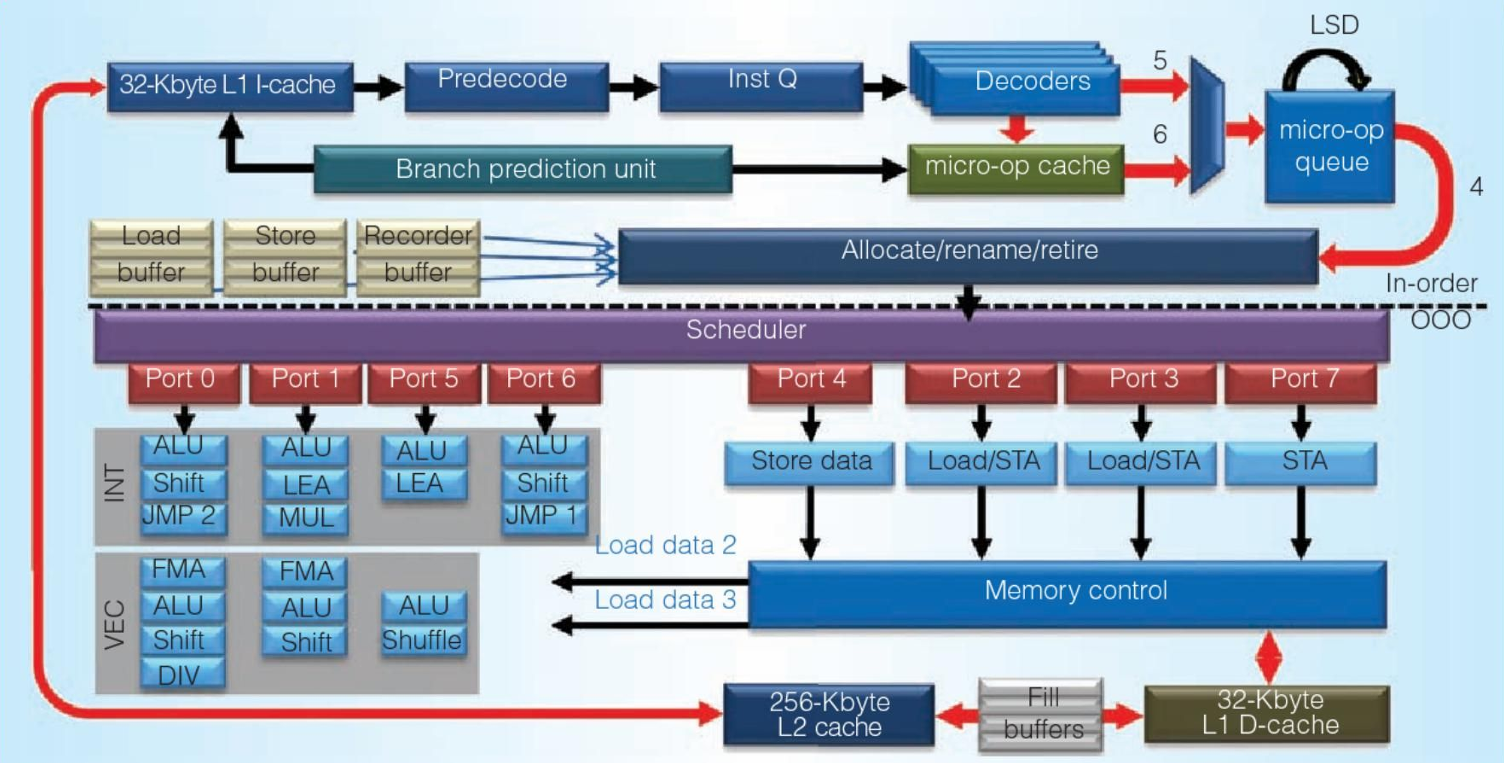
\includegraphics[width=0.7\linewidth]{Images/cap_4/cpu_superscalari.png}
\end{figure}
La capacità superscalare di questo tipo di CPU è data dall'avere diverse \textbf{porte di accesso} per mandare in esecuzione le istruzioni e diverse unità logiche per eseguirle. Notiamo una divisione in:
\begin{itemize}
    \item \textbf{Front\-End:} è la parte che recupera le istruzioni dalle cache le decodifica, predice i branch e smista le istruzioni sulle diverse porte.
    \item \textbf{Back\-End}: è la parte responsabile dell'esecuzione effettiva delle istruzioni e della riscrittura in memoria nel caso in cui sia necessario. Questa parte si occupa anche di gestire l'esecuzione delle operazioni \textbf{out-of-order} a seconda delle dipendenze che possono esserci.
\end{itemize} 
\subsection{Pipeline di Esecuzione}
La operazioni effettuate dalla nostra CPU seguono in realtà una serie di passaggi ben definiti:
\begin{itemize}
    \item \textbf{Fetch}: fase in cui vengono richiamate le istruzioni dalla memoria/cache.
    \item \textbf{Decode}: fase in cui l'istruzione è interpretata e compresa.
    \item \textbf{Esecuzione}: in cui l'operazione viene eseguita.
    \item \textbf{Writeback}: fase in cui il risultato deve essere registrato in memoria.
\end{itemize}
Queste operazioni possono essere eseguite da una singola istruzione per volta e, chiaramente richiedono un certo tempo per essere eseguite. Per evitare di dover aspettare che ogni singola istruzione finisca la Pipeline, facciamo sì che ogni istruzione sia in un certa fase diversa della pipeline, così da per aumentare il \textbf{throughput}. 
Un altro modo per ottimizzare la pipeline è quello di utilizzare \textbf{pipeline multiple} che si dividono in base al tipo di istruzione che è necessario effettuare. Infatti, abbiamo detto che esistono varie unità di esecuzione che sono indipendenti tra di loro e che, quindi, possono lavorare in parallelo. 
\begin{figure}[H]
    \centering
    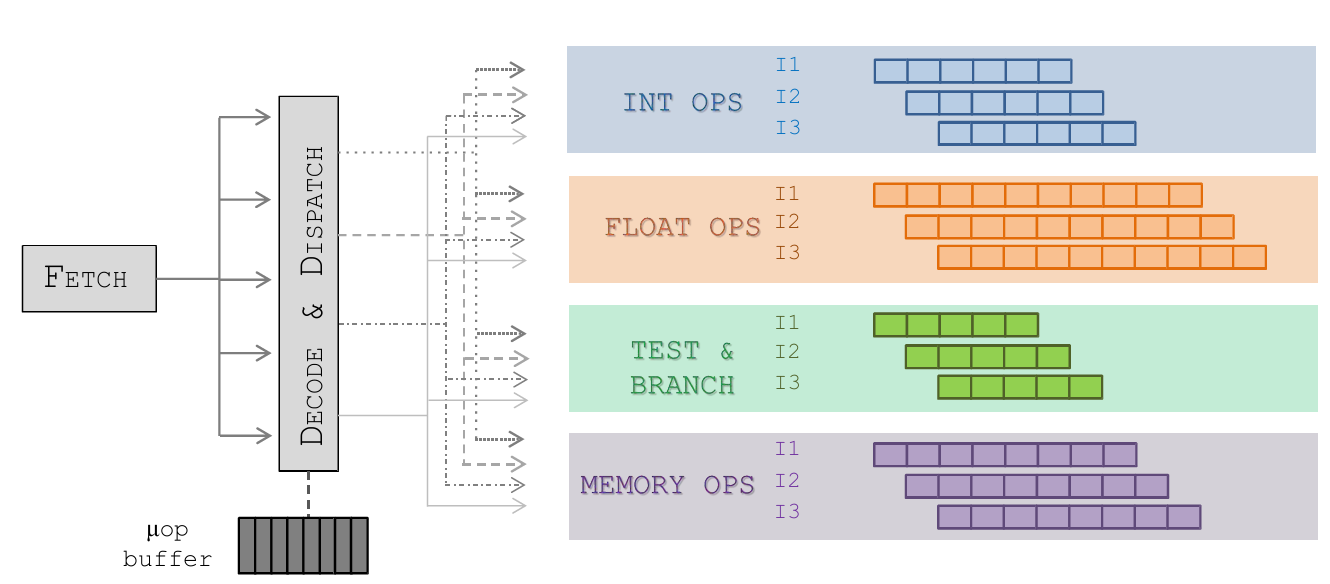
\includegraphics[width=0.7\linewidth]{Images/cap_4/pipeline_multiple.png}
\end{figure}

Il pipelining è sicuramente ottimo quando le istruzioni sono tutte indipendenti l'una dalle altre, tuttavia introducono alcuni problemi:

\begin{enumerate}
    \item \textbf{Data hazard}: un'istruzione dipende dal risultato di un'istruzione precedente che non ha ancora completato la pipeline. \textbf{Soluzione}: La CPU deve inserire stalli (bubble) nella pipeline, perdendo cicli produttivi.
    \item \textbf{Control hazard}: quando la CPU incontra un branch condizionale, non sa quale ramo eseguirà finché non valuta la condizione, ma nel frattempo la pipeline ha già iniziato a fare il prefetch delle istruzioni successive.
    \textbf{Soluzione}: branch predictor, un componente hardware che cerca di indovinare quale ramo verrà preso, basandosi sulla storia dei branch precedenti.
\end{enumerate}

Infine, un ulteriore ottimizzazione viene introdotta alla fine degli anni '90 con i \textbf{registri vettoriali}. Questi sono grandi registri nella CPU che permettono di eseguire una singola istruzione su tutti gli elementi del registro vettoriale in parallelo.
Infine, all'inizio degli anni 2000 troviamo che i sistemi sono dotati di più core avvicinandoci quindi alla struttura più comune a oggi. 

\section{Evitare le Inefficienze}
Scrivere codice pulito e logico è il prerequisito fondamentale per scrivere del buon codice, tuttavia, per ottenere le massime prestazioni da esso è necessario evitare inefficienze legate a salti, pipeline, cicli e controlli condizionali. Esistono cinque regole pratiche da applicare durante la stesura del codice.
\subsection{Esempio che seguiremo}
Supporremo di avere una distribuzione di punti casuali in un punto 2D che è diviso in sottoregioni. Per ogni punto, vogliamo selezionare tutte le celle della griglia il cui centro è più vicino a p di un certo raggio r ed eseguire su di esse alcune operazione.
Partiamo, dunque, da questo codice:
\begin{framed}
\begin{minipage}{\textwidth}
\footnotesize % Riduce la dimensione del carattere per guadagnare spazio
\begin{verbatim}
for (p = 0; p < Np; p++) {
    for (i = 0; i < Ng; i++) {
        for (j = 0; j < Ng; j++) {
            for (k = 0; k < Ng; k++) {
                dist = sqrt(
                pow(x[p] - (double)i/Ng + half_size, 2) +
                pow(y[p] - (double)j/Ng + half_size, 2) +
                pow(z[p] - (double)k/Ng + half_size, 2)
                );
                if (dist < R) {
                    fai_qualcosa;
                }
            }
        }
    }
}
\end{verbatim}
\end{minipage}
\end{framed}

\subsection{1. Evitare Chiamate a Funzioni Costose}
Alcune chiamate a funzioni, sono parecchie costose anche a causa del doversi collegare a delle librerie esterne. In questo codice, ad esempio, poiché calcoliamo la distanza tra vari punti, troviamo la funzione \textit{pow} e la funzione \textit{sqrt} per fare il quadrato e la radice. 
Notiamo che possiamo anche evitare questa cosa poiché ci basta considerare la distanza al quadrato dato che, alla fine, ci basta che vengano presi quegli specifici punti. Inoltre, sappiamo che i computer non sono molto bravi a effettuare le operazioni di divisione poiché hanno la necessità di calcolare l'inverso. Per evitare questo, possiamo precalcolarlo se è necessario effettuare la divisione più volte.
Infine, poiché $(double)i * Ng_inv + half_size$ è indipendente dal punto preso, possiamo anche questo, precalcolarlo in un array.
\begin{framed}
\noindent
\footnotesize
\begin{verbatim}
for (i = 0; i < Ng; i++) {
    for (j = 0; j < Ng; j++) {
        for (k = 0; k < Ng; k++) {
            dx = x[p] - (double)i * Ng_inv + half_size; 
            dy = y[p] - (double)j * Ng_inv + half_size; 
            dz = z[p] - (double)k * Ng_inv + half_size;
            
            dist2 = dx*dx + dy*dy + dz*dz;
            if (dist2 < R2) {
                /* fai qualcosa */ 
            }
        }
    }
}
\end{verbatim}
\vspace{0.3cm}
\end{framed}
Nella versione presenta, ancora non è stata ancora inserita l'ultima ottimizzazione.
\subsection{2. Hoisting delle espressioni}
Guardando il codice precedente, possiamo soffermarci su alcuni specifici calcoli. Infatti, nel ciclo più interno noi calcoliamo $dx$ e $dy$ senza che questi dipendano effettivamente da $k$. Per quanto questo possa sembrare semplicemente una scelta per non rendere il codice confusionario, in realtà provoca grossi ritardi a causa del fatto che questi vengono calcolati $k$ volte più del necessario. Possiamo dunque spostarli nel ciclo più in alto così da evitare questo problema.
\begin{framed}
\footnotesize
\begin{verbatim}
double ijk[Ng];
for (i = 0; i < Ng; i++) {
    ijk[i] = (double)i * Ng_inv + half_size; // Pre-calcolo
}

for (i = 0; i < Ng; i++) {
    dx2 = x[p] - ijk[i];
    dx2 = dx2 * dx2; // Spostato nel ciclo 'i' 
    
    for (j = 0; j < Ng; j++) {
        dy2 = y[p] - ijk[j];
        dy2 = dy2 * dy2;
        dist2_xy = dx2 + dy2; // Spostato nel ciclo 'j'
        
        for (k = 0; k < Ng; k++) {
            dz = z[p] - ijk[k];
            dist2 = dist2_xy + dz * dz; // Solo questo in k
            
            if (dist2 < Rmax2) { /* fai qualcosa */ }
        }
    }
}
\end{verbatim}
\end{framed}
\subsection{3. Chiarire lo Scope delle Variabili}
Nell'esempio considerato, troviamo delle variabili che sono funzionali alla specifica operazione che stiamo facendo. In particolare ci riferiamo a $dx,dy,dz$ e $dist$. Una cosa che possiamo fare è andare a definirle all'interno stesso del ciclo in cui vengono utilizzate. Questo aiuta di molto il compilatore che sa con certezza che non è necessario conservarne il valore al di fuori di quelle parentesi.
\begin{framed}
\footnotesize
\begin{verbatim}
for(int i = 0; i < Ng; i++) {
    // dx2 vive solo all'interno del ciclo 'i'
    double dx2 = x[p] - (double)i * Ng_inv + half_size; 
    dx2 *= dx2; 
    
    for(int j = 0; j < Ng; j++) {
        // dy2 e dist2_xy vivono solo qui
        double dy2 = y[p] - (double)j * Ng_inv + half_size; 
        double dist2_xy = dx2 + dy2 * dy2; 
        
        for(int k = 0; k < Ng; k++) {
            // dz e dist2 vivono solo qui
            double dz = z[p] - (double)k * Ng_inv + half_size; 
            double dist2 = dist2_xy + dz * dz; 
            
            if (dist2 < Rmax2) { 
                // fai qualcosa con sqrt(dist2); 
            }
        }
    }
}
\end{verbatim}
\end{framed}
\subsection{4. Suggerisci cosa è Importante}
Quando una variabile viene calcolata e riutilizzata frequentemente all'interno di un loop critico, può essere utile suggerire al compilatore di dedicarle un registro hardware utilizzando la parola chiave \texttt{register}. È fondamentale ricordare che si tratta solo di un \textbf{suggerimento non vincolante}: il compilatore, dopo aver analizzato il codice, potrebbe comunque decidere una strategia di allocazione diversa a causa di ragionamenti interni suoi sul come avrà intenzione di gestire la pipeline.
\subsection{5. Non ripetere controlli o referenziazioni non necessarie}
Spesso, anche a causa delle nostre abitudini di lavoro, ci ritroviamo spesso a ripetere dei controlli che spesso sono ridondanti rispetto a quello che già controlliamo. Infatti, questo è dovuto al fatto che la maggior parte delle volte siamo convinti di fare un bene al nostro codice rendendolo più sicuro quando, in realtà, non stiamo facendo altro che rallentarlo. Vediamo un esempio:
\begin{framed}
\noindent
\footnotesize
\begin{verbatim}
char * find_char_in_string( char *string, char c )
{
    int i = 0;
    // strlen() viene chiamata a ogni iterazione
    while ( i < strlen(string) ) {
        if ( string[i] == c )
            break;
        else
            i++;
    }
    if ( i < strlen(string) )
        return &string[i];
    else
        return NULL;
}
\end{verbatim}
\end{framed}
In questo caso, il problema di performance è causato dal fatto che \texttt{strlen} attraversa l'intera stringa a ogni ciclo per calcolarne la lunghezza, portando a una complessità quadratica. La stringa, ovviamente, non cambia nel corso delle iterazioni, dunque, ha senso calcolarla prima così da non ripetere una chiamata a funzione esterna.
Esistono due soluzioni parecchio interessanti:
\begin{framed}
\footnotesize
\begin{verbatim}
//V.1 La lunghezza è pre-calcolata 
int i = 0;
int len = strlen(string);
while (i < len) {
    if(string[i] == c) break;
    else i++;
}

//V.2 Controllo del terminatore tramite puntatori 
char *pos = string;
while((*pos != '\0') && (*pos != c)) 
    pos++;
return (*pos == '\0'?NULL:pos);
\end{verbatim}
\end{framed}
Simile è quello che accade con questa funzione riguardo alla referenziazione della memoria:
\begin{framed}
\footnotesize
\begin{verbatim}
// Accesso in memoria ad ogni iterazione
void reduce_vector(int n, double *array, double *sum) {
    for (int i = 0; i < n; i++) *sum += array[i]; 
    // Scrive e legge l'indirizzo di 'sum' N volte
}
\end{verbatim}
\end{framed}
L'introduzione di un accumulatore locale separato permette di sfruttare i registri veloci della CPU, limitando la scrittura in memoria a una sola istruzione una volta terminato il ciclo:
\begin{framed}
\footnotesize
\begin{verbatim}
// Uso di un accumulatore locale 
void reduce_vector(int n, double *array, double *sum) {
    double temp = 0; // Variabile locale
    for (int i = 0; i < n; i++) {
        temp += array[i]; // Elaborazione veloce e locale
    }
    *sum = temp; // Un solo accesso in memoria 
}
\end{verbatim}
\end{framed}
\subsection{Avvertenza su Numeri in Virgola}
Si potrebbe pensare che un compilatore con un alto livello di ottimizzazione (es. \texttt{-O3}) sia sempre in grado di riorganizzare i calcoli matematici per renderli più convenienti ma \textbf{questo non è vero per i numeri in virgola mobile}.

Mentre l'aritmetica intera in complemento a 2 è commutativa e associativa, la matematica in virgola mobile non è mai associativa:
\begin{equation}
    (a+b)+c \neq a+(b+c)
\end{equation}

A causa del numero limitato di cifre (precisione finita), l'ordine delle operazioni altera il risultato finale. Ad esempio, considerando una precisione limitata, sommare $1.00 + 0.001$ restituisce $1.00$, causando una perdita del decimale che invece non si avrebbe sommando prima i numeri più piccoli. Di conseguenza, il compilatore \textbf{non rimescolerà mai l'ordine delle operazioni floating point}, costringendo lo sviluppatore a scrivere direttamente la forma algebrica più efficiente nel codice sorgente.

\section{Ottimizzazione basata sulla Cache}
Abbiamo già visto la cache e il motivo della sua introduzione per risolvere il problema del \textbf{Memory Wall} e abbiamo già parlato della \textbf{gerarchia di memoria} che questa introduce.
Per cercare di capire come ottimizzare al meglio l'utilizzo della cache ripetiamo adesso i due principi fondamentali:
\begin{itemize}
    \item \textbf{Località temporale}: dati referenziati di recente vengono spesso riutilizzati.
    \item \textbf{Località spaziale}: dati vicini in memoria vengono spesso referenziati insieme.
\end{itemize}
Teniamo bene a mente questi due principi per capire comprendere al meglio le scelte che vengono prese nella mappatura della cache.
\subsection{Mappatura della Cache}
Supponiamo che la memoria RAM e la cache siano divisi in \textbf{blocchi} di uguale dimensione. Quando andremo a spostare un blocco in cache, non sposteremo dunque il singolo bit, bensì tutto il singolo blocco.
\begin{figure}[H]
    \centering
    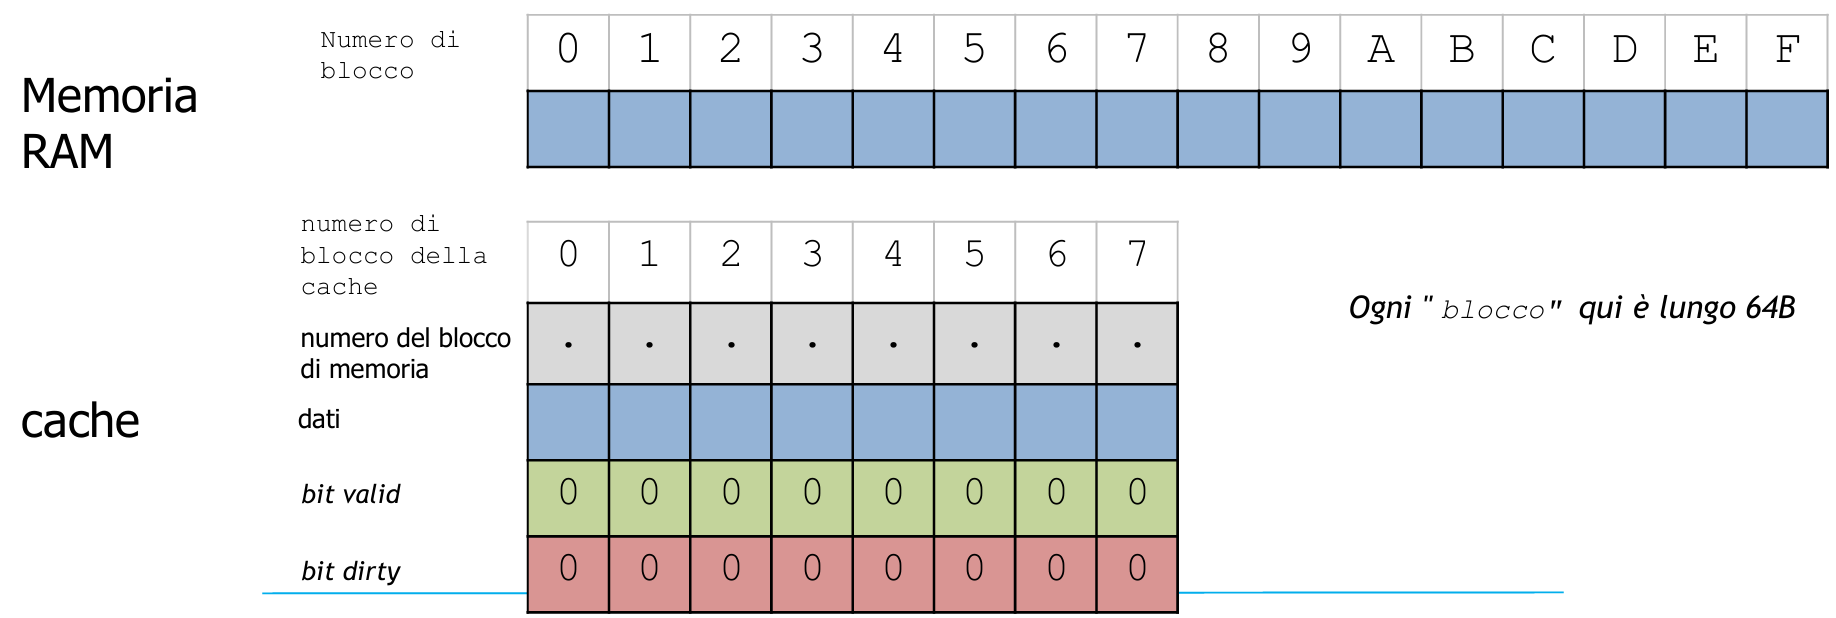
\includegraphics[width=0.7\linewidth]{Images/cap_4/cache_vs_ram.png}
\end{figure}
In cache oltre ai blocchi in sé per sé troviamo:
\begin{itemize}
    \item \textbf{bit valid:} che è un bit che ci indica se quel dato è ancora valido o se non è più presente nella RAM e, quindi, può essere anche eliminato nella cache se necessario.
    \item \textbf{bit dirty:} è un bit che ci indica che il dato presente in cache è stato modificato rispetto al dato presente in RAM e che, quindi, è necessaria una scrittura quando possibile. Possono esserci due strategie riguardo a questo bit, la prima è che si scrive sempre sulla RAM una volta che il dato è stato modificato la seconda è che si posticipa la scrittura in RAM fino a quando si può. La seconda opzione è consigliata quando si hanno tanti cambiamenti di dati così da non dover fare molte scritture.
\end{itemize}

Tornando alla mappatura da memoria RAM a cache troviamo le seguenti strategie:
\begin{itemize}
    \item \textbf{Completamente associativa}: I dati possono andare in qualsiasi blocco libero. È efficiente per evitare conflitti in scrittura, ma lenta in lettura perché richiede la ricerca in tutta la cache.
    \item \textbf{Mappatura diretta}: Un indirizzo RAM può risiedere in un solo specifico blocco. Estremamente veloce da trovare, ma massimizza i conflitti se più dati utili competono per lo stesso blocco.
    \item \textbf{Set-associativa a N-vie}: È il compromesso tipico delle architetture moderne (es. associativa a 8 vie). I dati possono essere inseriti in uno specifico sottoinsieme (set) di blocchi.
\end{itemize}
Per scrivere codice efficiente bisogno gestire le tre C e le tre R:
\begin{itemize}
    \item \textbf{Compulsory miss} $\rightarrow$ Inevitabili al primo accesso.
    \item \textbf{Capacity miss} (Spazio insufficiente) $\rightarrow$ Si contrasta con la regola \textbf{Ridurre}: usare tipi di dati più piccoli e lavorare su working set limitati.
    \item \textbf{Conflict miss} (Sovrascrittura di linee cache utili) $\rightarrow$ Si contrasta con le regole \textbf{Riorganizzare} (layout di memoria per migliorare la località) e \textbf{Riutilizzare} (completare tutte le operazioni su un dato mentre è ancora residente in cache).
\end{itemize}
\subsection{Modello di accesso alla Memoria}
Le prestazioni della memoria formano una superficie tridimensionale nota come \textit{Memory Mountain}, che dipende strettamente da due fattori: la \textbf{dimensione del \textit{working set}} (quanti dati stiamo manipolando) e lo \textbf{Stride} (il "passo" con cui leggiamo gli elementi in memoria). 

Lavorare con un set di dati piccolo e uno stride unitario (elementi contigui) massimizza la banda passante (\textit{Bandwidth}). Al contrario, scorrere grandi array saltando posizioni di memoria (stride elevato) distrugge le prestazioni perché spreca le linee di cache caricate.
\begin{framed}
\footnotesize
\noindent
\textbf{Esempio: Impatto dello Stride nell'Accesso alla Memoria} \\
La CPU non carica in cache singoli elementi interi, ma intere linee da 64 byte. Nel primo ciclo (\texttt{stride = 1}), un singolo accesso alla RAM carica in cache un blocco che contiene anche gli elementi successivi, rendendo le iterazioni seguenti istantanee. 

\begin{verbatim}
#define N 1000000
int a[N];
int sum = 0;

/* Accesso sequenziale (Stride = 1) */
/* Veloce: sfrutta appieno l'intera cache line*/
for (int i = 0; i < N; i++) {
    sum += a[i];
}
\end{verbatim}

\vspace{0.3cm}
\noindent
Se incrementiamo l'indice in modo non sequenziale, stiamo ignorando i dati portati in cache. Ad ogni salto, la CPU va in \textit{cache miss} ed è costretta a pagare la penalità di centinaia di cicli per interrogare nuovamente la RAM.

\begin{verbatim}
/* Accesso sparso (Stride grande) */
/* Lento: spreca quasi tutta la cache line e genero miss*/
for (int i = 0; i < N; i += 16) {
    sum += a[i];
}
\end{verbatim}
\end{framed}
Questo principio diventa critico quando si opera su \textbf{matrici multidimensionali}. In linguaggi come C e C++, le matrici non sono tabelle magiche, ma blocchi unidimensionali e continui di memoria. La convenzione di questi linguaggi è il \textbf{row-major order} (ordine per righe): gli elementi della stessa riga sono memorizzati consecutivamente in RAM. Al contrario, leggere una matrice scorrendola per colonne significa effettuare salti enormi (\textit{stride}) nella memoria fisica, abbattendo radicalmente le prestazioni del programma (uno \textit{stride} pari a $N \times S$ byte, dove $N$ è la dimensione della riga e $S$ la dimensione del dato).
\begin{figure}[H]
    \centering
    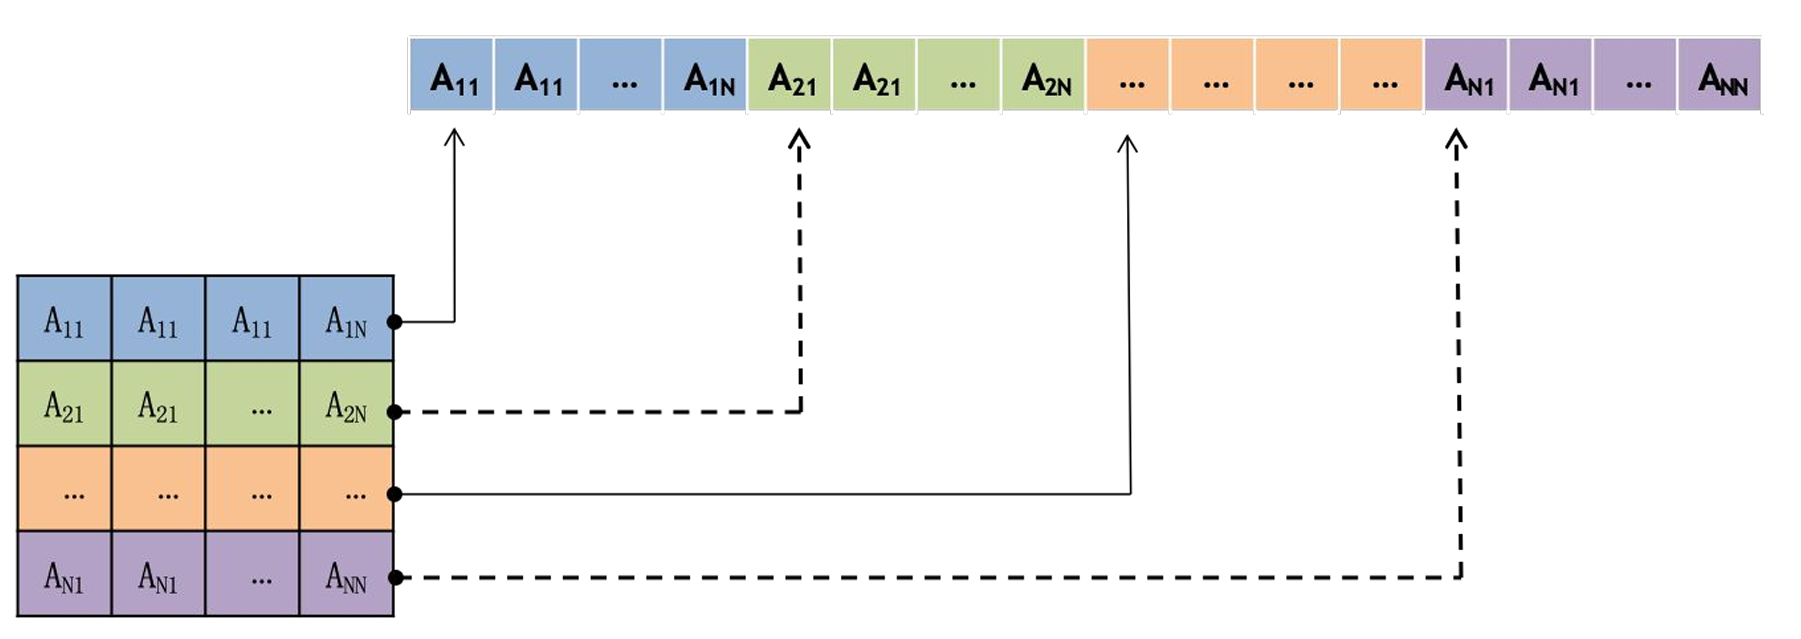
\includegraphics[width=0.7\linewidth]{Images/cap_4/matrice_in_memo.png}
\end{figure}
La lettura della matrice quindi per colonne è chiaramente estremamente costosa dato che è necessario effettuare grandi salti andando quindi a passare da un punto della memoria a un altro anche provocando molti cache miss.
\begin{figure}[H]
    \centering
    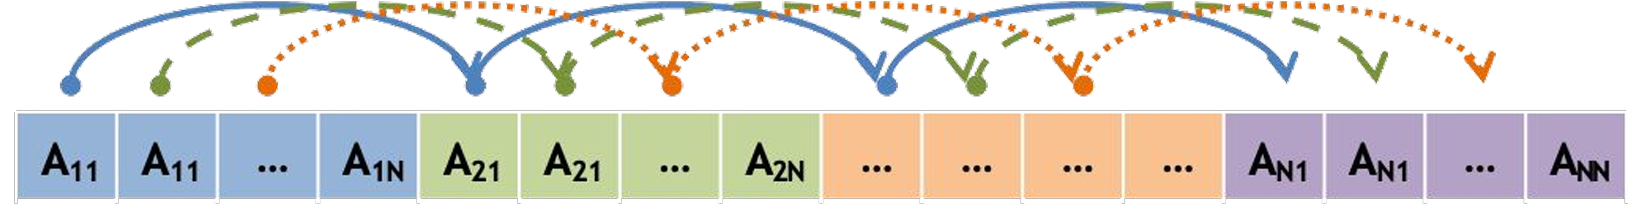
\includegraphics[width=0.5\linewidth]{Images/cap_4/lettura_colonne.png}
\end{figure}
In genere, l'indice interno è quello che varia più velocemente e traccia la contiguità della memoria e, quindi, abbiamo che $M[i][j][k]$ è contiguo a $M[i][j][k+1]$.
Considerando tutto quello che abbiamo detto, analizziamo questa sezione di codice:
\begin{framed}
\footnotesize
\noindent
\textbf{Esempio: Lettura vs Scrittura con Stride} \\
Nel primo caso leggiamo in modo contiguo ma scriviamo a salti. Nel secondo caso scriviamo in modo contiguo ma leggiamo a salti.

\begin{verbatim}
// Modalità 1: Lettura contigua, Scrittura con stride
for(int row = 0; row < N; row++) {
    for(int col = 0; col < N; col++) {
        A[col * N + row] = B[row * N + col];
    }
}

// Modalità 2: Scrittura contigua, Lettura con stride
for(int row = 0; row < N; row++) {
    for(int col = 0; col < N; col++) {
        A[row * N + col] = B[col * N + row];
    }
}
\end{verbatim}
\end{framed}
In entrambi i casi abbiamo uno stride, tuttavia, questi non sono uguali. Quando si modifica il contenuto di una variabile, tale modifica equivale a sovrascrivere una posizione di memoria. Quando la variabile viene caricata nella memoria cache, ciò che viene caricata è una copia della variabile, che mantiene la sua posizione originale nella memoria principale. Quindi, se modifichiamo il suo valore, dobbiamo modificarlo solo nella cache o anche nella memoria principale?
\begin{itemize}
    \item \textbf{Write-Through}: La modifica viene scritta immediatamente sia in cache che in RAM mantenendoli coerenti.
    \item \textbf{Write-Back}: La modifica viene apportata solo in cache e la RAM viene aggiornata solo quando la linea di cache viene sostituita.
\end{itemize}
In caso di \textit{write-miss} in una cache di tipo write-through possiamo allocare prima il blocco in cache e poi effettuare la scrittura in entrambi (write-allocate) o scrivere direttamente sulla memoria principale (non-write-allocate). Nell'ultimo caso la scrittura a raffica è conveniente per evitare continue allocazioni in cache.
\subsection{Organizzazione dei Dati}
Poiché lavoriamo con cache che hanno generalmente dimensioni molto piccole, organizzare i dati per far sì che questi stiano dentro la cache diventa fondamentale per sfruttare il principio di località spaziale.
\subsubsection*{Scansione per blocchi}
Oltre alla classica scansione per righe/colonne esiste un altro tipo di scansione detta \textbf{scansione per blocchi} fatta appositamente per essere sfruttata quando lavoriamo con operazioni molto pesanti come moltiplicazioni o inversioni di matrice. L'idea è che invece di attraversare intere righe o colonne, dividiamo la matrice in \textbf{sottomatrici più piccole} dette blocchi scegliendo la dimensione facendo sì che i blocchi delle matrici coinvolte siano tutti in cache così da abbattere i cache miss.
\begin{figure}[H]
    \centering
    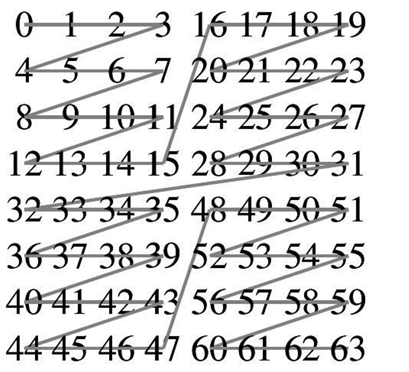
\includegraphics[width=0.25\linewidth]{Images/cap_4/lettura_blocchi.png}
\end{figure} 

Anziché codificare manualmente la dimensione del blocco, è possibile memorizzare direttamente la matrice in RAM utilizzando pattern non lineari, come la \textbf{Curva di Morton} (o Z-order).  Questo ordinamento mappa dati multidimensionali in 1D mantenendo fisicamente vicini in memoria i punti che sono vicini nello spazio 2D o 3D, migliorando le prestazioni medie su architetture diverse senza bisogno di un \textit{tuning} manuale dei blocchi.
\subsubsection*{Campi Caldi e Campi Freddi}
Un errore comune nell'ottimizzazione è progettare strutture dati (\texttt{struct}) che mescolano dati ad accesso frequente ("caldi") con dati raramente utilizzati ("freddi"). Nelle liste concatenate, ad esempio, i puntatori e le chiavi di ricerca vengono letti ad ogni iterazione, mentre il carico utile (payload) viene letto solo in caso di successo.

\begin{framed}
\footnotesize
\noindent
\textbf{Esempio: Ottimizzazione delle Strutture Dati} \\
Nella prima versione, l'inserimento di un grosso array tra la chiave e il puntatore al nodo successivo allontana fisicamente i due dati. Questo distrugge la località spaziale: la cache verrà inondata da byte inutili caricati per via del payload (\texttt{my\_data}).

\begin{verbatim}
// Versione NON ottimizzata (Campi mischiati)
struct my_node {
    double key;            // HOT
    char my_data[300];     // COLD: Allontana key e next 
    my_node *next_node;    // HOT
};
\end{verbatim}
\end{framed}
La soluzione consiste nell'estrarre i dati "freddi" in una struttura separata allocata altrove, lasciando nella struttura principale solo un puntatore. In questo modo, \texttt{key} e \texttt{next\_node} diventano adiacenti in memoria e verranno caricati insieme in una singola e veloce linea di cache.
\begin{framed}
\footnotesize
\begin{verbatim}
// Versione OTTIMIZZATA (Separazione Hot/Cold)
struct my_data {
    char data[300];
};

struct my_node {
    double key;            // HOT
    my_node *next_node;    // HOT: Ora è adiacente alla chiave!
    struct my_data *payload; // COLD: Puntatore ai dati esterni
};
\end{verbatim}
\end{framed}

\section{Branch condizionali}
Ogni volta che la sequenza di operazioni da eseguire o i dati da elaborare dipendono da una condizione (ad esempio, l'esito di un test 'if'), il programma effettua un'esecuzione condizionale. Le architetture moderne gestiscono questa situazione a basso livello in due modi distinti: modificando il flusso di controllo oppure modificando il flusso di dati.

\subsection*{Flusso di Controllo}
A livello macchina, il controllo viene passato a una sezione diversa del codice tramite istruzioni di salto (\textit{jump}). Queste possono essere:
\begin{itemize}
    \item \textbf{Incondizionate} (\texttt{jmp}): Il salto avviene sempre.
    \item \textbf{Condizionali} (\texttt{je, jne, jg, jl, ecc.}): L'esecuzione dipende dall'esito di un test precedente. Queste istruzioni leggono i bit del \textbf{registro dei flag} (es. \textit{Zero Flag, Sign Flag, Carry Flag}), che memorizza lo stato dell'ultima operazione logico-aritmetica.
\end{itemize}
In questo scenario, il codice generato dal compilatore è pieno di bivi e diramazioni fisiche.

\subsection*{Flusso di Dati}
Le CPU moderne offrono un meccanismo alternativo: invece di saltare a blocchi di codice diversi, calcolano in anticipo i possibili risultati e poi spostano nei registri finali solo il dato corretto (es. Tramite l'istruzione assembly \texttt{cmov} - \textit{conditional move}).
Questo approccio non genera bivi nel codice, mantenendo un flusso di esecuzione lineare e altamente prevedibile. Tuttavia, è applicabile solo a scenari semplici poiché altrimenti il numero di operazioni necessarie al calcolo supera il vantaggio dato dal calcolare tutti i risultati.
\subsection{Branch Predictor}
Per mantenere le pipeline di esecuzione sempre piene, le CPU utilizzano un componente hardware chiamato \textbf{Branch Predictor}, che cerca di indovinare in anticipo l'esito di una diramazione prima che questa venga effettivamente valutata per anticiparne i calcoli.

I migliori predittori moderni hanno un'accuratezza del $95\%$. Tuttavia, quando il predittore sbaglia (\textbf{Branch Miss} o \textit{Misprediction}), la CPU è costretta a svuotare l'intera pipeline scartando il lavoro fatto in anticipo. Questa penalità costa tipicamente dai 10 ai 30 cicli di clock per ogni errore.

L'impatto statistico è enorme: supponiamo di avere un blocco di 140 istruzioni in cui 1 istruzione su 7 è un branch (quindi 20 branch in totale). Assumendo eventi indipendenti, la probabilità che la pipeline \textit{non} venga mai svuotata con un predittore accurato al $95\%$ crolla drasticamente:

\[P(no flush) = 0.95^{20} \approx 0.3585 \Rightarrow 35.85\%\]


Con un predittore al $90\%$, la probabilità scende ad appena il $12.16\%$. Per questo motivo, i branch condizionali all'interno dei cicli (\textit{loop}) sono i nemici principali delle prestazioni e vanno evitati o ristrutturati.

Ecco perché la seconda strategia che abbiamo visto, la modifica condizionale del flusso di dati, è preferibile quando possibile e il compilatore cercherà di utilizzarla il più possibile poiché non genera istruzioni di salto e il flusso di esecuzione è lineare e perfettamente prevedibile. Tuttavia, come abbiamo detto, si applica solo a un limitato sottoinsieme di casi.

Una cosa da tenere in considerazione che provoca un miglioramento delle prestazioni è che il branch con la condizione vera è quello che sta più vicina rispetto all'if stesso. Dunque, per evitare salti da una parte all'altra del codice, sarebbe bene che il branch vero sia quello che è più probabile che venga utilizzato.

Idealmente vorremmo evitare i branch condizionali il più 
possibile all'interno dei cicli:
\begin{itemize}
    \item Spostandoli fuori da Loop e scrivendo Loop più specializzati.
    \item Esecuzioni di variabili/quantità impostate fuori dal ciclo.
    \item Utilizzando puntatori alle funzioni invece di selezionare funzioni all'interno di un ciclo.
    \item Uso di operazioni diverse per evitare branch.
\end{itemize}
\subsection{Tecniche per limitare i Branch}
In genere ci sono due casi possibili:
\begin{itemize}
    \item Le variabili testate nelle condizioni non cambiano durante il ciclo. Questo è il caso semplice e con poca ristrutturazione si hanno grandi miglioramenti.
    \item Le variabili cambiano nel ciclo. Qui abbiamo bisogno di molto lavoro in più per cercare di risolvere il problema.
\end{itemize}
Vediamo adesso una carrellata di esempi.
\subsubsection*{Sollevamento del loop}
Se una condizione testata all'interno di un ciclo non dipende dall'iteratore, è un grave errore ripeterla ad ogni passo. La diramazione va spostata \textit{fuori} dal ciclo, scrivendo versioni specializzate del loop stesso.
\begin{framed}
\footnotesize    
\begin{verbatim}
// Versione NON ottimizzata: il test viene ripetuto 'top' volte
for(int i = 1; i < top; i++) {
    if (value > 1) do_something();
    else           do_something_else(); 
}

// Versione OTTIMIZZATA: il test viene eseguito UNA sola volta
if (value > 1) {
    for (int i = 1; i < top; i++) do_something();
} else {
    for (int i = 1; i < top; i++) do_something_else(); 
}
\end{verbatim}

\vspace{0.3cm}
\noindent
\textit{Nota:} Nei casi di scelte multiple basate su uno stato costante, è nettamente preferibile usare un costrutto \texttt{switch} invece di una cascata di \texttt{if/else}. Il compilatore traduce lo \texttt{switch} in una tabella statica di puntatori detta \textbf{jump table} a cui si accede in tempo costante $O(1)$ senza diramazioni condizionali.
\end{framed}
\subsubsection*{Flussi di dati imprevedibili}
Quando la condizione dipende dai dati stessi (es. l'elemento corrente di un array casuale), il predittore fallirà continuamente. Spesso si può sostituire l''if' con un'operazione booleana moltiplicativa.
\begin{framed}
\footnotesize    
\begin{verbatim}
// Versione NON ottimizzata: Rischio altissimo di Branch Miss
for (int i = 0; i < SIZE; i++) {
    if (data[i] > PIVOT) 
        sum += data[i];
}

// Versione OTTIMIZZATA: Nessun salto! Il flusso è lineare.
for (int i = 0; i < SIZE; i++) {
    sum += (data[i] > PIVOT) * data[i];
}
\end{verbatim}
\end{framed}
Poiché $(data[i] > PIVOT)$ viene valutato come 1 (Vero) o 0 (Falso), è possibile sfruttare questa logica per eliminare il branch.
\subsubsection*{Ordinamento degli elementi}
Un caso classico è lo scambio condizionale di valori tra due array per mantenere un ordinamento. L'uso esplicito dell''if' distrugge le prestazioni. È preferibile usare operatori condizionali ternari o maschere bit a bit che il compilatore può tradurre in istruzioni \texttt{cmov} (flusso di dati condizionale senza salti).
\begin{framed}
\footnotesize

\begin{verbatim}
// Versione NON ottimizzata
for (int i = 0; i < SIZE; i++) {
    if (A[i] < B[i]) {
        int t = B[i];
        B[i] = A[i];
        A[i] = t;
    }
}

// Versione OTTIMIZZATA: Sfrutta min e max
for (int i = 0; i < SIZE; i++) {
    int min = (A[i] > B[i]) ? B[i] : A[i];
    int max = (A[i] >= B[i]) ? A[i] : B[i];
    
    A[i] = max;
    B[i] = min;
}
\end{verbatim}
\end{framed}
\subsubsection*{Cambiare il POV}
A volte il modo migliore per rimuovere i branch è ripensare i limiti stessi dei cicli, invece di usare `if` interni per discriminare le aree spaziali (es. in una matrice). 

Vogliamo riempire la diagonale di una matrice $M \times N$ con $0.0$, il triangolo superiore con $1.0$ e quello inferiore con $-1.0$.
\begin{framed}
\footnotesize

\begin{verbatim}
// Versione NON ottimizzata: if/else dentro i loop annidati
for (int j = 0; j < N; j++) {
    for (int i = 0; i < M; i++) {
        if (i > j)       matrix[j][i] = 1.0;
        else if (i <= j) matrix[j][i] = -1.0;
        else             matrix[j][i] = 0.0;
    }
}

// Versione OTTIMIZZATA: Loop separati basati sulla geometria
for (int j = 0; j < N; j++) {
    int i;
    for (i = 0; i < j; i++)        // Fino alla diagonale
        matrix[j][i] = -1.0;
        
    matrix[j][i] = 0.0;            // Sulla diagonale esatta
    
    for (i = j + 1; i < M; i++)    // Dopo la diagonale
        matrix[j][i] = 1.0;
}
\end{verbatim}
\end{framed}
\section{Ottimizzazione dei Loop}
Ottimizzare i cicli significa massimizzare il riutilizzo dei dati e mantenere le pipeline della CPU sempre piene. 
Per capire quanto un ciclo sia ottimizzabile, si introduce il concetto di \textbf{Intensità Aritmetica ($A_I$)}, definita come il rapporto tra il numero di operazioni eseguite $f(n)$ e la quantità di dati trasferiti $n$:
\begin{equation}
    A_I = \frac{f(n)}{n}
\end{equation}
In base all'intensità aritmetica, i cicli si classificano in tre categorie:
\begin{enumerate}
    \item \textbf{$O(N)/O(N)$}: Es. Addizioni vettoriali o prodotti scalari. Il potenziale di ottimizzazione è limitato perché il limite è imposto dalla larghezza di banda della memoria. Le migliorie derivano dall'evitare accessi ripetuti (es. \textit{Loop Fusion}).
    \item \textbf{$O(N^2)/O(N^2)$}: Es. Moltiplicazione matrice-vettore. Offre maggiori opportunità di ottimizzazione sfruttando la località spaziale e temporale.
    \item \textbf{$O(N^3)/O(N^2)$}: Es. Moltiplicazione matrice-matrice. Ha un enorme potenziale di ottimizzazione perché i dati caricati in cache possono essere riutilizzati molteplici volte per fare calcoli.
\end{enumerate}
\subsection{Ottimizzazioni per Cicli a Bassa Intensità: Loop Fusion}
Quando si elaborano cicli $O(N)/O(N)$, l'obiettivo principale è ridurre il traffico verso la memoria principale. Se due cicli consecutivi scorrono gli stessi array, fonderli in un unico ciclo (\textbf{Loop Fusion}) dimezza i caricamenti dalla RAM.

\begin{framed}
\noindent
\footnotesize
\textbf{Esempio: Fusione dei Loop (Loop Fusion)}
\begin{verbatim}
//B[i] viene caricato dalla RAM due volte
for(int i=0; i<N; i++) 
    A[i] = B[i] * C[i];
for(int i=0; i<N; i++) 
    Q[i] = B[i] + D[i];

//OTTIMIZZATA: Fusione, B[i] è letto una sola volta.
for(int i=0; i<N; i++) {
    A[i] = B[i] * C[i];
    Q[i] = B[i] + D[i];
}
\end{verbatim}
\end{framed}

\subsection{Ottimizzazioni per Cicli $O(N^2)$: Unroll \& Jam}
Nei cicli annidati, è possibile ridurre l'overhead e migliorare il riutilizzo dei dati srotolando il ciclo esterno e fondendolo con quello interno (\textbf{Unroll \& Jam}). 

Tuttavia, bisogna prestare attenzione al \textbf{Register Spilling}: se si srotola troppo (es. un fattore $m$ troppo grande), la CPU esaurisce i registri hardware disponibili ed è costretta a riversare continuamente i dati temporanei nella cache, rallentando drasticamente il calcolo (\textit{codice gonfiato}).

\begin{framed}
\footnotesize
\noindent
\textbf{Esempio: Unroll \& Jam in una Moltiplicazione Matrice-Vettore}
\begin{verbatim}
// 1. Versione Base (3*N^2 accessi)
for(int i=0; i<N; i++)
    for(int j=0; j<N; j++)
        C[i] += A[i][j] * B[j];

// 2. Non accediamo a C[i] ma a una variabile locale
for(int i=0; i<N; i++) {
    double c_temp = C[i];
    for(int j=0; j<N; j++)
        c_temp += A[i][j] * B[j];
    C[i] = c_temp;
}

// 3. Unroll & Jam
for(int i=0; i<N; i+=2) {
    for(int j=0; j<N; j++) {
        double b_temp = B[j];
        C[i]   += A[i][j]   * b_temp;
        C[i+1] += A[i+1][j] * b_temp;
    }
}
\end{verbatim}
\end{framed}

\subsection{Srotolamento del Ciclo (Loop Unrolling) e Aritmetica Floating Point}
Lo srotolamento (\textit{unrolling}) è una trasformazione fondamentale che espone il parallelismo a livello di istruzione (ILP) e riduce il costo di aggiornamento del contatore.

Esiste però un'enorme differenza tra variabili intere e in virgola mobile. Come discusso in precedenza, \textbf{la matematica in virgola mobile non è associativa}. Se si compila una semplice somma di array (`S += A[i]`) usando il tipo \texttt{int}, il compilatore vettorizza automaticamente il codice massimizzando le prestazioni. Se si usa il tipo \texttt{double}, il compilatore \textbf{non} ottimizzerà il ciclo, perché alterare l'ordine delle somme cambierebbe il risultato numerico a causa degli arrotondamenti. È quindi responsabilità del programmatore riassociare esplicitamente le operazioni.

\begin{framed}
\noindent
\footnotesize
\textbf{Esempio: Srotolamento e Riassociazione Esplicita per i Double} \\
Per sfruttare le porte vettoriali della CPU con i `double`, dobbiamo srotolare manualmente il ciclo e forzare un nuovo ordine di valutazione tramite le parentesi, esponendo operazioni indipendenti.

\begin{verbatim}
// la CPU deve aspettare la fine della somma precedente
for (int i=0; i<N; i++)
    S = S + A[i];

// Versione Srotolata 2x1 
//(Riduce l'overhead del ciclo, ma resta sequenziale)
for (int i=0; i<N-2; i+=2)
    S = (S + A[i]) + A[i+1];

// Versione Srotolata e RIASSOCIATA (Parallelismo esposto!)
for (int i=0; i<N-2; i+=2)
    S = S + (A[i] + A[i+1]);
\end{verbatim}
\vspace{0.3cm}
\noindent
\textit{Nota:} Modificando l'ordine in `(A[i] + A[i+1])`, le due somme elementari sono indipendenti dal valore precedente di `S`. La CPU può calcolare questo blocco in parallelo nelle proprie pipeline vettoriali (es. istruzioni AVX \texttt{vaddpd}) e sommarlo ad `S` solo alla fine, abbattendo drasticamente il tempo di esecuzione. Ricordarsi sempre di gestire la "coda" (tail) del ciclo per gli elementi residui non multipli del fattore di srotolamento.
\end{framed}

\subsection{Esempio Pratico $O(N^3)/O(N^2)$: Moltiplicazione Matrice-Matrice (MMM)}
La moltiplicazione di due matrici quadrate $C = A \times B$ richiede $2N^3$ operazioni floating point (flop). A causa dell'ordine \textit{row-major} del linguaggio C, attraversare la matrice $B$ per colonne provoca un'enorme quantità di \textit{cache miss}. Un'implementazione ingenua genera quasi un cache miss per ogni flop, degradando le prestazioni.

Esistono tre fasi progressive per ottimizzare questo problema computazionale:
\begin{enumerate}
    \item \textbf{Trasposizione preventiva}: Trasporre la matrice $B$ in memoria prima dei calcoli permette di accedere ad entrambe le matrici sequenzialmente (per righe).
    \item \textbf{Scambio dei cicli (Loop Swapping)}: Cambiare l'ordine di annidamento dai classici \texttt{i-j-k} a \texttt{i-k-j}. Questo approccio accede agli elementi di $C$ in modo contiguo e legge $B$ in ordine di riga, riducendo le letture dalla RAM.
    \item \textbf{Elaborazione a Blocchi (Tiling)}: Mantenere in cache sottomatrici fisse (blocchi o \textit{tiles}). Invece di calcolare un'intera riga per volta, si accumulano risultati parziali su un blocco ristretto di $C$ sfruttando mini-porzioni di $A$ e $B$ caricate in L1. 
\end{enumerate}

\textbf{Impatto sulle metriche:} I profiler hardware dimostrano che passando dall'implementazione ingenua (\texttt{O0 naive}) all'implementazione a blocchi (\texttt{O3 tailed}), i miss della cache L1 crollano vicino allo zero, l'IPC (Instructions Per Cycle) si avvicina al massimo teorico dell'architettura e il tempo di esecuzione scala perfettamente senza subire crolli all'aumentare di $N$.
